\section{Available Projects}
This is a list of available projects. Of course, you can still select your own topic as described in Section \ref{sec:SelectOwnTopic}, or, if you want to do the same topic as another group, propose changes to the lecturer for approval.

\subsection{SF - Smoothing Filter}
Send the src address and len to indicate the starting address of an input sample and its length in words. Also send a dest value to indicate where the smoothed value is to be stored. Toggle the activate bit to perform the smoothing (i.e., could do an average of m elements). The SF sets it done bit to true when complete. An example of the smoothing process is shown in Figure \ref{fig:smooth_sg2} below.

\begin{figure}[H]
\centering
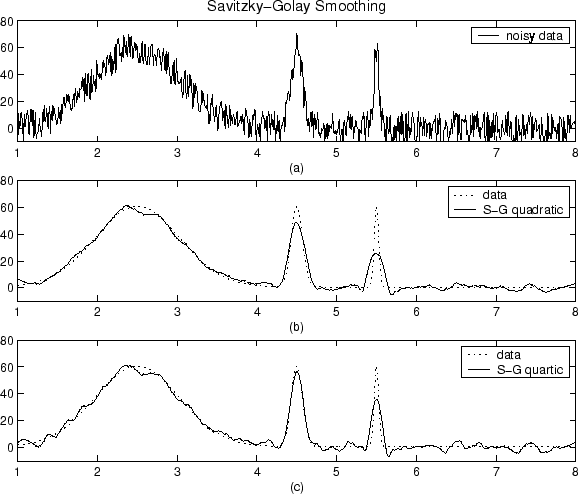
\includegraphics[width=0.6\columnwidth]{Figures/smooth_sg2}
\caption{Smoothing Filter}
\label{fig:smooth_sg2}
\end{figure}


\textbf{Inputs:} unsigned src, unsigned len, unsigned dest, bit activate\\
\textbf{Output:} bit done

\subsection{CAM - Content Addressable Memory}
Consider a table where each element has the form defined as follows:
\begin{lstlisting}
 struct TableElement{
  unsigned key;
  byte record[rsize];
 };
\end{lstlisting}

The table itself is in the form:
\begin{lstlisting}
 struct TableElement table[nelements];
\end{lstlisting}

The CAM accelerator is sent the partial contents of a record and it returns the key, if found. If the contents is not found, the value 0xFFFFFFFF is returned. The user can ask the CAM accelerator to continue searching and find the next occurrence of the given search string.

The rsize member is constant for each element in a table, but multiple tables may exist with different rsize values for each table. The CAM accelerator must be able to store table start index and rsize information so that subsequent uses of the CAM accelerator, when using the same table, does not need to resend the table addressing information.

\textbf{Inputs:} unsigned start, unsigned rsize, unsigned nelements, bit activate, byte array search string\\
\textbf{Output:} unsigned key, bit done, bit found

\subsection{SFI - Sampled Function Interpolator}

Store a function as follows:
\begin{lstlisting}
Fy = array[0...N]
Fx = array[0..N]
\end{lstlisting}
Fx[i] will contain an x values corresponding to y value Fy[i]. 

So the sampling of the funding might not be consistent (eg. parts may have more detail, the x values might be closer together than other parts; sometimes something like this can be useful e.g. where a function has more complex behaviour at a turning point)

The function  \verb|gety(x)|,  which you are meant to implement, will search in Fx to find the closest x. If that exact x is found at say i, then it will return Fy[i]. Otherwise if x is between Fx[i] and Fx[i+1], you will need to return an interpolation of Fy[i] and Fy[i+1].  For a simple starting point, it could just be the average of the two points, although of course this would not be so accurate. Ideally, it should rather calculate which Fy is closer and do a calculation based on the distance.


% Tell the SFI the start address and len of a src float array to upsample, tell the IF the dst array that is 2x(end-start) elements, tell the IF to start. The IF then adds a value between each sample of src, saving the new sample in array dst (and sets done to true when finished). i.e. the C code would look like this:
% \begin{lstlisting}
%  int j = 0;
%  for(i = 0; i < len-1; i++){
%   dst[j  ] = src[j];
%   dst[j+1] = src[j] + (dst[j+1] - src[j]) / 2.0;
%   j += 2;
%  }
% \end{lstlisting}

% As an optional advanced option: make the dst array length Nx(end-start) elements, where N is any positive integer.

\textbf{Inputs:} unsigned start, unsigned dst, unsigned len, bit start\\
\textbf{Outputs:} bit done

\subsection{PRNG - Parallel Random Number Generator}
Generate N random numbers in one go. The idea is that the PNRG could write directly to RAM, and a soft processor can access it. Generates numbers in range 0 to $2^{32}-1$.

For this project, you need to consider ways in which to interface the PRNG to RAM, which you could implement as an array of 32-bit unsigned values that has a dual-port interface (covered in the lectures, but good example code available at \href{http://www.asic-world.com/examples/verilog/ram_dp_sr_sw.html}{this link}).

\textbf{Inputs:} unsigned seed, unsigned start\_address, unsigned count (i.e. the number of random numbers to generate), bit activate\\
\textbf{Output:} bit busy

\subsection{DM - Delta Modulator}
Send a stream of 8 bytes to the DM device, and it returns 1 byte, where the bits in sequence from lsb to msb represents the delta modulation.

The delta modulator is pretty easy, so you might want to add additional features, for example:

\textbf{Optional extra feature 1:} Make the LEDs on the FPGA board indicate the half wavelength (e.g. for a sinusoidal signal, the delta value is only going to change at the turning points, so counting the number of inputs from one change in delta to the next, and showing that number of the LEDs, will give a approximation for the wavelength).

\textbf{Optional extra feature 2:} Add flow control. Assume that the DM might take a long time to complete. So, in this case, the processor needs to wait for the DM to be ready for input, then send the input, waits for the result, and then goes back to waiting for the DM to be ready for more input. You could add pushbutton control to either clock the DM or to control how fast it is clocked. The combination of Extra feature 1 and 2 will make it easier for humans to see the LEDs display wave length information.

\textbf{Inputs:} byte byteIn, bit clock\\
\textbf{Output:} modOut


\subsection{ASG - Arithmetic Series Generator}
This accelerator generates the series:
\begin{lstlisting}
a(n) = a1 + (n-1)d 
\end{lstlisting}


The inputs saddr indicates the starting address in memory where the generated sequence is to be stored. A activate input bit will be needed to tell the ASG to start processing; the ASG will return done when complete.

\textbf{Inputs:} float a1, float d, unsigned n, unsigned saddr, bit activate\\
\textbf{Outputs:} done


\subsection{SALG - Selection Address List Generator}
The SALG is sent the starting address of a table in memory. The table has n elements. Each element of the table is in the form TableElement shown below. The SALG is sent a second address, called inds, which it will use to store the addresses (i.e., the starting address of the relevant record field) that matches the selection criteria (which is hardcoded).
\begin{lstlisting}
struct TableElement{
    unsigned key;
    byte record[rsize];
};
TableElement table[n];
\end{lstlisting}

Example implementation of SALGA function that returns the address of all records that have odd numbered keys:

\begin{lstlisting}
 void SALGA(TableElement* table, unsigned* inds, unsigned n){
  unsigned n_inds = 0;
  for(int i = 0; i < n; i++){
   if(table[n]->key & 1)
    inds[n_inds++] = &table[n]->record[0];
  }
  inds[n_inds] = 0; // set last one to null to indicate end of list
 }
\end{lstlisting}
As is the case with the other accelerators, an activate input and done output would be needed.

\textbf{Inputs:} unsigned table, unsigned n, unsigned inds, bit activate\\
\textbf{Outputs:} bit done


\subsection{FSG - Function Samples Generator}
The FSG is used to generate a sequence of samples from a hard-coded function. The FSG is given two float inputs, xstart and xend, which indicates the range for the x values that you want to samples for the function, as well as an unsigned nsamp input indicating the number of samples you want to obtain. A fourth parameter, p, indicates the memory address to write the sampled values to.

The FSG implements a FPGA equivelent of the following C code. Note that the function fn would be hard-coded, it's just easier to show a function there to help the explanation in C.

\begin{lstlisting}
 void FSG(float xstart, float xend, unsigned nsamp, float* p){
  unsigned i;
  done = 0; // clear the done signal
  for(i = 0; i < nsamp; i++){
   p[i] = fn(xstart + i*(xend-xstart) / nsamp);
  }
  done = 1; // raise the done signal to indicate to the
            // softprocessor that the operation is finished
 }
 
 float fn(float x){
  // This example just returns a polynomial
  return 5*x*x + 3*x;
 }
\end{lstlisting}

\textbf{Inputs:} float xstart, float xend, unsigned nsamp, float* p, bit activate\\
\textbf{Outputs:} bit done

\subsection{BSS - Bit Sequence Sniffer}
The Bit Sequence Sniffer (BSS) device is connected onto a series binary data transmission line, for example a RS232 data line or (with an appropriate differential signal demodulator unit) onto data lines of a USB connector. A "sniffer" device has many real-world applications, and these type of things exist in reality.

``Data sniffers" can generally be divided into a variety of types, such as: transmission line sniffers, debug sniffers, security sniffers, self-diagnostic sniffer module. Transmission line sniffers are perhaps the most general case; these could for example simply record data that is sent along data lines - these would generally be used for reputable purposes such as monitoring utilisation levels of connections. Debug sniffers could for instance be JTAG-like devices that could be used to gain useful debugging data, for example checking that the bits sent from an ADC to the CPU are all successfully obtained by the CPU. Security sniffers have many applications, for example to detect threats to a network (e.g., a computer jamming the network with junk messages, or probing attacks from an unrecognised IP or stack overflow attacks).

Basic sniffers are not particularly complex pieces of equipment, but they generally need to operate at high speed in order to capture the bits of data. For this project, the objective is to develop a RS232 transmission line sniffer that will be able to connect to either the RX or TX line and be able to capture bytes of data sent. To simplify things, the protocol can be assumed to be something easy like one start bit, 8 data bits, 1 parity and 1 stop bit (i.e., 11 bits per 8 bytes of data sent). Added to this should be detecting a particular sequence, say a series of bytes such as \{0xA0, 0xB5, 0xFF\}; and if such a sequence is detected, then a LED flashes. If time permits, a more sophisticated version could be constructed that detects a start sequence (e.g., 0xA0) and then captures the next 10 bytes and sends them out the USB / debug channel to be displayed on the attached PC.

A small breadboard circuit will likely be needed in order to adjust voltage levels for the sniffer if one of the PIO pin on the FPGA is going to be used to sense the input.

You may use something like a USB to UART converter and PuTTY to generate data for the FPGA to sniff.

Notes on inputs and outputs:
\begin{itemize}
    \item SniffIn\\
    This would be the input bit connected to one of the RS232 RT/TX data lines.
    \item Seqdetect\\
    Output bit (to turn on LED also) to record that a pre-programmed sequence was detected.
    \item DataOut\\ 
    Ability to dump a suspect sequence to a connected PC for recording (i.e., for if the last part of the description above is implemented).
\end{itemize}


\subsection{BCDC - Binary Coded Decimal Converter}
\textbf{TODO: Change slightly?}

The BCDC converts a binary integer of arbitrary length to a sequence of binary coded decimal digits. Inputs to the device are a starting address, input src, and len indicating the number of bytes to convert. A third input dst indicates the address where the converted values are stored. As with the other proposed projects, when the active input changes from low to high, the BCDC starts, and then raises the done output to indicate completion.

\textbf{Notes on inputs and outputs:}

Assume the input integer 2 882 400 018 (0xABCDEF12 hex). This input is 4 bytes long and the output is 10 nibbles (5 bytes): array bcd = {0010, 1000, 1000, 0010, 0100, 0000, 0000, 0000, 0001, 1000} // note each element is in base 2

It is your choice to use either little endian or big endian representation.

\subsection{NCSM - Nonlinear Check Sum Module}
Most check-sums are simple, just summing each input value, call it x(n) that comes in; so the function would read something like y = Sum x(n) for n = 1..n.

This project aims to experiment with nonlinear check-sums functions as a means to create a check value that is perhaps more robust but also more platform specific. The NCSM project probably sounds quite simple, and for the most part is. It implements 32-bit fixed point calculations of the input steam of bytes sent to the NCSM module. If you'd prefer a more intense challenge (that would also improve performance and look more impressive), then attempt to do the checksum on a block of RAM memory. The nonlinear function, called funct below must be implemented to account for wrapping and suitable use of mapping a 8-bit input to the 32-bit output range.

The implementation in C-style pseudo-code is as follows:
\begin{lstlisting}
 unsigned funct(input byte x, output unsigned y){
  y = 100*sin((x-128)*M_PI/32);
 }
 
 void checksum(
  input  byte     x,
  input  bit      reset,
  input  bit      clk,
  output unsigned result
 ){
  static unsigned sum = 0;
  if(reset clocked){
   sum = 0;
   return;
  }
  if(clk clocked){
   sum   += funct(input, n);
   result = sum;
  }
 }
\end{lstlisting}
A graph of the suggested funct is provided below in Image \ref{fig:NCSM}.

\begin{figure}[H]
\centering
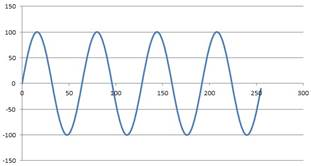
\includegraphics[width=0.6\columnwidth]{Figures/NCSM}
\caption{Suggested Function Graph}
\label{fig:NCSM}
\end{figure}

\textbf{Inputs:} unsigned x, bit reset, bit clk\\
\textbf{Outputs:} unsigned result

\subsection{MD5 - Message Digest Version 5}
MD5 is a standard hashing algorithm most frequently used to verify the contents of large files against unintentional corruption. For example, if you've downloaded a large file and want to ensure that it downloaded correctly.  MD5 was initially designed to be used as a cryptographic hash function, but it has been found to suffer from extensive vulnerabilities. It remains suitable for other non-cryptographic purposes, for example for determining the partition for a particular key in a partitioned database. More information can be found on \href{https://en.wikipedia.org/wiki/MD5}{Wikipedia}.

\textbf{Inputs:} stream of data to be verified\\
\textbf{Outputs:} unsigned MD5 sum

\subsection{MMA - Matrix Multiplier Accelerator}
The MMA works on square matrices (if you feel inspired, you can revise it to work on appropriately sized rectangular matrices). Two memory addresses are passed to MMA, namely A and B, in indicate the starting addresses of the matrices to be multiplied. A third memory address, C indicates the address to save the resultant matrix. Input n indicates the size of the matrices. Assume the matrices contain floats. Assume that the matrix elements are indexed in the standard way, i.e.:

index of A(i, j) = j*n + i (where i and j are in the range 0 to n-1)

The activate bit input will be clocked to tell the MMA to start multiplying. The MMA will raise the done output high when it is complete.

\subsection{IMA - Image Masking Accelerator}
The IMA overlays an image mask on a larger image by using the XOR operation. Assume both the mask and the larger image are in RGB 12-bit color (4-bit per component) uncompressed format, at a resolution of 320 x 240. The result is displayed on a VGA screen.

It is strongly suggested that you start by getting the VGA output on the FPGA to work. Tutorials can be found on the Digilent Website. \href{https://reference.digilentinc.com/learn/programmable-logic/tutorials/nexys-4-vga-test-pattern-with-mouse-overlay/start}{Here's an example for the Nexys 4.} 

You can get creative with the image mask you choose to apply.

\begin{table}[H]
\centering
\caption{Inputs and Outputs for the Image Masking Accelerator}
\label{tbl:IMAIO}
\begin{tabular}{ll}
\textbf{Input} & \textbf{Explanation} \\ \hline
\multicolumn{1}{|l|}{mask} & \multicolumn{1}{l|}{address of the image mask in memory} \\ \hline
\multicolumn{1}{|l|}{mw, mh} & \multicolumn{1}{l|}{width and height in pixels of the mask} \\ \hline
\multicolumn{1}{|l|}{mx, my} & \multicolumn{1}{l|}{(x, y) offset from top left of image that the mask is to be applied} \\ \hline
\multicolumn{1}{|l|}{img} & \multicolumn{1}{l|}{the image that the mask is to be overlaid} \\ \hline
\multicolumn{1}{|l|}{iw, ih} & \multicolumn{1}{l|}{the width and height in pixels of the image} \\ \hline
\multicolumn{1}{|l|}{activate} & \multicolumn{1}{l|}{bit input to be clocked to activate the IMA} \\ \hline
\textbf{Output} & \textbf{Explanation} \\ \hline
\multicolumn{1}{|l|}{done} & \multicolumn{1}{l|}{set high once the mask has been overlaid} \\ \hline
\end{tabular}
\end{table} 
Note: This project is designed with a Nexys 4 or better in mind, which has 4 860 kbit on-chip memory. For optimal RAM usage, the RAM blocks can be configured to have a word width of 36-bit.

\subsection{PSA - Pattern Seek Accelerator}
The PSA searches for a particular sequence of bytes in a block of memory.

\begin{table}[H]
\centering
\caption{Inputs and Outputs for the Pattern Seek Accelerator}
\label{tbl:PSAIO}
\begin{tabular}{ll}
\textbf{Input} & \textbf{Explanation} \\ \hline
\multicolumn{1}{|l|}{unsigned p} & \multicolumn{1}{l|}{the pattern to be searched for} \\ \hline
\multicolumn{1}{|l|}{unsigned pl} & \multicolumn{1}{l|}{length of the pattern in bytes} \\ \hline
\multicolumn{1}{|l|}{unsigned b} & \multicolumn{1}{l|}{address of the block of memory to searh} \\ \hline
\multicolumn{1}{|l|}{unsigned bl} & \multicolumn{1}{l|}{number of bytes in b} \\ \hline
\multicolumn{1}{|l|}{it activate} & \multicolumn{1}{l|}{clock to activate the PSA and tell it to continue searching from last address} \\ \hline
\multicolumn{1}{|l|}{bit reset} & \multicolumn{1}{l|}{set b and clock reset to tell the PSA to start searching from address b} \\ \hline
\textbf{Output} & \textbf{Explanation} \\ \hline
\multicolumn{1}{|l|}{bit done} & \multicolumn{1}{l|}{the PSA sets this to high when it is complete} \\ \hline
\multicolumn{1}{|l|}{unsigned found} & \multicolumn{1}{l|}{\begin{tabular}[c]{@{}l@{}}that the pattern started at (note that you might find it easier to set found to \\ pl + the start of the pattern that was found. found could be set to \\ 0xFFFFFFFF if nothing was found, otherwise you could add a success bit\\ to indicate if the pattern was found.\end{tabular}} \\ \hline
\end{tabular}
\end{table}

\textbf{Simplification:} if you want, you can simplify the topic. For example, the PSA could just respond with a found set to 1 or 0 depending whether the pattern was found. Further simplifications could be to look for a single byte in a block of memory (i.e., only using one address input, namely b).

\textbf{Example operation}
\begin{lstlisting}
Assume:

p = 0xFF00, pl = 2
b = 0xFF10, bl = 8
memory location 0xFF00 = {101, 102}
memory location 0xFF10 = {99, 100, 101, 102, 103, 101, 102, 100}
Steps:

First p will be reset
    PSA.b = 0xFF10; PSA.reset = 0; PSA.reset = 1; PSA.reset = 0;
Next the inputs are specified
    PSA.p = 0xFF00; PSA.pl = 2;
    PSA.b = 0xFF10; PSA.bl = 8;
The activate is clocked
    PSA.activate = 0; PSA.activate = 1; PSA.activate = 0;
The PSA now proceeds to do the first search
    PSA.done = 1; PSA.found = 0xFF12;
The PSA is clocked again to continue the search
    PSA.activate = 0; PSA.activate = 1; PSA.activate = 0;
Another match was found
    PSA.done = 1; PSA.found = 0xFF15;
The PSA is clocked again to continue the search
    PSA.activate = 0; PSA.activate = 1; PSA.activate = 0;
No more matches
    PSA.done = 1; PSA.found = 0xFFFFFFFF;
\end{lstlisting}


\subsection{DEA - Data Encryption Accelerator}
The objective the Data Encryption Accelerator (DEA) is to accelerate the process of encrypting a data stream. First the (reset) control line is clocked, this causes the DEA to reset any internal buffers and storage. Next, an encryption key is set by writing the (a single byte value) of the key to the din (data input) 8-bit data input bus, and then sending a positive edge to the kset (key set) control line. The dclk (data clock) is kept low. After this, the actual encryption starts, which involves iterating through all the data, one byte at a time, by writing a byte of data to the din input lines, then clock dclk clock line. The encrypted data is (pretty much) immediately available on the DEA's dout 8-bit output lines. The latter process is repeated for each item of data.

To start with, you could use simple XOR encryption. If time permits, you could then take it further using some sort of repeating pattern based on the key input.

\subsection{VADER - Versatile Accelerated Digital Encryption Recovery}
The VADER system is a digitally accelerated add-on hardware device designed to recover passwords using an acquired hashed password and hashing function. Uses of such a device could be to speed up computationally expensive recovery of passwords for forensic purposes such as instances where a victim or suspects password protected information could assist in an investigation. In order for the system to begin the specific hashing function used to create the password hashes would need to be acquired; it is assumed that this is available and many commonly used hashing functions are indeed widely available. The hashed version of the password itself would also need to be acquired. The system will run parallelised functions on an FPGA to accelerate the recovery of the password. The system will first run a dictionary type cracking attempt and following this if it is unsuccessful a brute force algorithm will be applied.

\subsection{ISD - Image Steganography Decoder}
Steganography is the practice of concealing a file, message, image, or video within another file, message, image, or video.

For this project, one passes an image into the module and it extracts an encoded message. The encoding might be hiding data in the least significant bit  (eg 8 pixels -> 1 8-bits piece of data). Of course there's a whole lot of other ways that one could do this. The encoding would likely happen on the PC, e.g. using Julia or another appropriate programming language. The iamge could be put as code in the HDL program, or loaded from the SD card if enough time is available. The module could then decode the message from the figure in memory and display the message either on the 7 segment display or the LEDs (could possibly using a combination of LEDs and 7seg to show text of a longer message).

To read more about steganography, visit \href{https://en.wikipedia.org/wiki/Steganography}{Wikipedia}.

\subsection{PADAWAN - Parallel Accelerator for Digitising Audio with Attenuation of Noise}
The problem to be solved is performing filtering and processing on audio in near real-time using an FPGA.

Real-time filtering can be achieved in software, however when many filters are cascaded one after the other (or in parallel in the case of an equaliser) there will be a delay between audio input and output. For many applications this is an undesirable side-effect, preventing the system from being considered real-time.

Some types of filters that can be implemented are: low-pass, high-pass, band-pass and band-stop. Some effects that can be implemented are: echo, flange, chorus, reverberation, vibrato, phaser, delay and distortion. The user should be able to change the filter and effect parameters (in real-time) and hear the effect on the audio output.

The PADAWAN system is provided with a digital audio stream and output is converted to analogue by means of pulse width modulation (PWM). If time permits, the output must also pass through a noise shaper in order to increase the apparent output resolution.

Note: This project is intended for Nexys 4, which has an on-chip ADC and on-board PWM filter.

\textbf{Inputs:} Audio stream, filter and effect parameters\\
\textbf{Output:} PWM audio

\subsection{DDS - Direct Digital Synthesis}
Direct digital synthesis is a digital signal processing technique by which arbitrary waveforms can be generated. The DDS module is given a waveform definition (in the form if a look-up table), a frequency word and an amplitude word.

For the purposes of this project, the output is in the audio frequency band and converted to analogue by means of pulse width modulation (PWM). If time permits, the output must also pass through a noise shaper in order to increase the apparent output resolution.

Implementation of this project will start with the generation of a variable-frequency saw-tooth signal, which will eventually become the input of the look-up table.

\textbf{Inputs:} waveform definition, unsigned frequency, unsigned amplitude\\
\textbf{Output:} PWM audio
